\section{Hasil dan Pembahasan}

\subsection{Representasi Konten dan Gaya pada CNN}

\begin{figure*}[b]
    \centering
    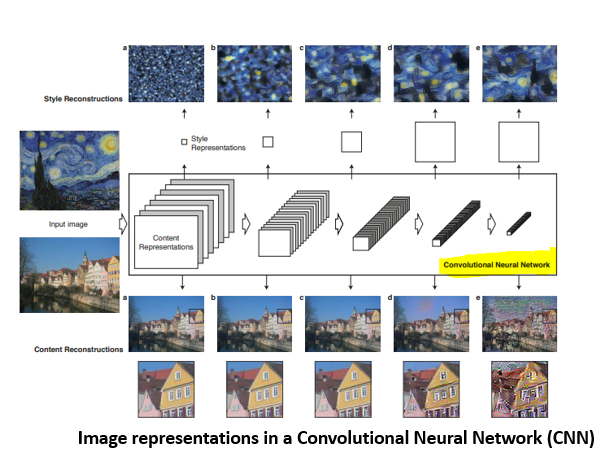
\includegraphics[width=0.5\textwidth]{assets/visualisasi-nst.png}
    \caption{\href{https://arxiv.org/pdf/1508.06576.pdf}{Visualisasi Proses NST}}
\end{figure*}

Pada algoritma \textit{Neural Style Transfer} (NST), \textit{Convolutional Neural Network} (CNN) berperan sebagai pemetaan dari piksel pada gambar ke fitur yang lebih memiliki makna. Setiap layer konvolusi dalam arsitektur VGG-19 menghasilkan himpunan \textit{feature map} yang dapat dipandang sebagai representasi berbeda dengan tingkat abstraksi yang meningkat seiring kedalaman layer. Secara umum, layer-layer awal cenderung menangkap pola lokal, seperti garis dan tekstur sederhana, sedangkan layer yang lebih dalam menangkap struktur global dan susunan objek dalam citra. 

Terdapat tiga buah citra utama yang penting, yaitu citra konten $I_c$, citra gaya $I_s$, dan citra hasil $I_g$. Citra konten $I_c$ adalah citra yang struktur semantiknya ingin dipertahankan, citra gaya $I_s$ adalah citra yang karakteristik artistiknya ingin ditransfer kepada citra $I_c$. Terakhir, citra hasil $I_g$ adalah citra yang menjadi variabel optimasi dan pada iterasi awal biasanya diinisialisasi sebagai citra konten $I_c$ atau citra noice acak.


Ketiga citra tersebut dimasukkan ke dalam jaringan VGG-19 yang bobotnya dibekukan, sehingga pada layer ke-$l$ masing-masing citra menghasilkan tensor fitur berdimensi berukuran $C_l \times H_l \times W_l$. Tensor-tensor ini kemudian di-\textit{flatten} dan dinyatakan sebagai matriks fitur
$$
F_c^l, F_s^l, F_g^l \in \mathbb{R}^{C_l \times (H_l \cdot W_l)}
$$
di mana tiap baris merepresentasikan satu kanal fitur dan setiap kolom merepresentasikan satu posisi spasial. Dengan demikian, pada layer ke-$l$, $F_c^l$ merupakan representasi fitur citra konten, $F_s^l$ merupakan representasi fitur citra gaya, dan $F_g^l$ merupakan representasi fitur citra hasil yang terus berubah seiring proses mengoptimasi $I_g$.

Pada representasi konten, informasi yang relevan adalah nilai aktivasi pada tiap posisi, sehingga jarak antara $F_c^l$ dan $F_g^l$ diukur langsung menggunakan norma Frobenius untuk mendefinisikan \textit{content loss}. Dengan demikian, konten dipandang sebagai pola aktivasi yang spesifik pada setiap lokasi dalam \textit{feature map}.

Dalam konteks pemisahan konten dan gaya, perbedaan karakteristik representasi ini dimanfaatkan untuk mendefinisikan dua jenis informasi yang ingin dipertahankan pada citra hasil $I_g$. Representasi konten biasanya diambil dari satu atau beberapa layer menengah yang dianggap cukup sensitif terhadap struktur global citra, tetapi tidak terlalu sensitif terhadap variasi tekstur lokal. Sebaliknya, representasi gaya diperoleh dari beberapa layer yang tersebar dari permukaan hingga kedalaman jaringan, sehingga dapat menangkap pola gaya pada berbagai posisi.


Berbeda dengan itu, representasi gaya diambil berdasarkan korelasi statistik antar fitur yang kemudian diringkas dalam bentuk Matriks Gram. Untuk setiap layer gaya ke-$l$, Matriks Gram $G_s^l$ dan $G_g^l$ dihitung dari $F_s^l$ dan $F_g^l$ sebagai
$$
G^l = F^l (F^l)^\top
$$
sehingga elemen $G_{ij}^l$ merepresentasikan inner product antara kanal ke-$i$ dan ke-$j$ yang mengukur tingkat keselarasan kedua fitur tersebut di seluruh posisi pada citra. Dengan cara ini, gaya tidak lagi bergantung pada posisi absolut di dalam citra, melainkan pada pola koaktivasi fitur yang bersifat lebih global. 

Pemilihan layer konten dan himpunan layer gaya tersebut tidak bersifat sembarang, melainkan dilihat dari pemahaman tentang bagaimana CNN menyandikan informai pada berbagai kedalaman jaringan. Layer yang terlalu dangkal jika digunakan sevagai representasi konten cenderung hanya mempertahankan detail lokal sehingga struktur semantik citra dapat terganggu, sedangkan layer gaya yang terlalu dalam berpotensi mengubah bentuk dalam porsi besar apabila Matriks Gram-nya dipaksakan untuk diikuti oleh citra hasil. Oleh karena itu, konfigurasi layer konten dan gaya dalam NST harus dipelajari secara mendalam sehingga kebutuhan mempertahankan struktur global citra konten dan karakteristik gaya dapat diseimbangkan dengan baik.


\subsection{Fungsi Loss pada Representasi Konten dan Gaya}
Setelah representasi konten dan gaya pada CNN didefinisikan melalui matriks fitur $F_c^l, F_s^l, F_g^l$ dan Matriks Gram, langkah berikutnya adalah menganalisis bagaimana fungsi loss membuat citra hasil $I_g$ mendekati citra konten dan citra gaya. Dalam konteks \textit{Neural Style Transfer} (NST), seluruh perilaku algoritma ditentukan oleh \textit{content loss}, \textit{style loss}, dan fungsi antar keduanya.

Representasi konten diambil dari matriks fitur $F_c^l$ dan $F_g^l$ pada layer ke-$i$, Secara intuitif, \textit{content loss} mengukur seberapa besar perbedaan antara citra hasil dan citra konten pada ruang fitur tersebut. Bentuk umum yang digunakan adalah
$$
\mathcal{L}_{content}^l = \frac{1}{2} \Vert F_g^l - F_c^l \Vert_F^2
$$

Jika $\mathcal{L}_{content}$ besar, berarti pola aktivasi $F_g^l$ berbeda jauh dari $F_c^l$, sehingga struktur objek dalam citra hasil mulai menyimpang dari citra konten. Sebaliknya, meminimalkan \textit{content loss} akan mendorong $F_g^l$ mendekati $F_c^l$, sehingga bentuk dan tata letak objek utama tetap terjaga. 

Berbeda dengan konten, gaya direpresentasikan melalui Matriks Gram yang menangkap korelasi antar fitur pada beberapa layer gaya yang dipilih. Untuk sebuah layer gaya ke-$l$, Matriks Gram $G_s^l$ dari citra gaya dan $G_g^l$ dari citra hasil didefinisikan dengan
$$
G_s^l = F_s^l (F_s^l)^\top, \hspace{1cm} G_g^l = F_g^l (F_g^l)^\top
$$
Lalu, \textit{style loss} pada layer tersebut kemudian diukur sebagai
$$
\mathcal{L}_{style}^l = \Vert G_g^l - G_s^l \Vert_F^2
$$
yang merepresentasikan seberapa jauh korelasi fitur citra hasil menyimpang dari korelasi fitur gaya. Nilai $\mathcal{L}_{\text{style}}^l$ yang kecil menunjukkan bahwa pola tekstur, warna, dan koaktivasi fitur pada $I_g$ mirip dengan $I_s$, terlepas dari posisi spasial gaya tersebut.

Dalam praktiknya, gaya tidak hanya diambil dari satu layer, tetapi dari himpunan layer $\mathcal{S}$ yang tersebar dai awal hingga akhir jaringan untuk menangkap gaya pada berbagai skala. \textit{Style loss} total biasanya dirumuskan sebagai
$$
\mathcal{L}_{style} = \sum_{l \in \mathcal{S}} w_l \mathcal{L}^l_{style}
$$

dengan $w_l$ adalah bobot kontribusi layer ke-$l$. Pemilihan dan pembobotan layer mempengaruhi seberapa halus atau kasarnya tekstur gaya yang muncul pada citra hasil.

Terakhir, untuk menghasilkan citra baru yang gayanya diambil dari $I_s$ dan kontennya dari $I_c$. Fungsi loss total biasanya ditulis dengan
$$
\mathcal{L}_{total} (I_g) = \alpha \mathcal{L}_{content}(I_g) + \beta \mathcal{L}_{style} (I_g)
$$

dengan $\alpha > 0$ dan $\beta > 0$ adalah hiperparameter yang mengatur keseimbangan antara preservasi konten dan intensitas gaya. Nilai $\alpha$ yang relatif besar akan menekankan kesesuaian konten, sehingga citra hasil cenderung mempertahankan struktur $I_c$ tetapi mungkin hanya mengadopsi gaya secara halus. Sebaliknya, nilai $\beta$ yang jauh lebih besar mendorong citra hasil untuk mengikuti Matriks Gram citra gaya secara agresif, sehingga tekstur dan warna gaya menjadi dominan tetapi struktur konten bisa mengalami distorsi.

\subsection{Optimasi Hasil Fungsi Loss terhadap Akurasi Citra Hasil Akhir}
Setelah \textit{content loss} dan \textit{style loss} dirumuskan, rekayasa citra hasil $I_g$ dilakukan melalui optimasi iteratif berbasis gradien terhadap piksel $I_g$. Ide utama dari menemukan \textit{content loss} dan \textit{style loss} minimum adalah dengan memperlakukan $I_g$ sebagai variabel bebas yang diubah sedikit demi sedikit sehingga $\mathcal{L}_{content}(I_g)$ dan $\mathcal{L}_{style}(I_g)$ sama-sama mengecil dan citra hasil menjadi semakin mirip dengan konten dan gaya yang diinginkan.

Optimasi menggunakan gradien ini digunakan dengan cara menghitung gradien total terhadap $I_g$ yang dihitung dengan menggunakan langkah-langkah berikut.
\begin{IEEEenumerate}
    \item Nyatakan gradien total sebagai penjumlahan berbobot gradien komponen konten dan gaya:
    $$
      \nabla_{I_g} \mathcal{L}_{\text{total}}
        = \alpha \, \nabla_{I_g} \mathcal{L}_{\text{content}}
        + \beta \, \nabla_{I_g} \mathcal{L}_{\text{style}}.
    $$
\item Hitung masing-masing gradien $\nabla_{I_g} \mathcal{L}_{\text{content}}$ dan $\nabla_{I_g} \mathcal{L}_{\text{style}}$ dengan menggunakan turunan parsial dan aturan rantai, yaitu dengan \textit{backtracking} gradien dari ruang fitur dan Matriks Gram kembali ke ruang piksel $I_g$ melalui jaringan CNN. ($\partial \frac{\mathcal{L}_{total}}{\partial I_g}$)
    \item Perbarui $I_g$ sedikit ke arah $-\nabla_{I_g} \mathcal{L}_{\text{total}}$ untuk menurunkan nilai loss. Secara umum, pembaruan ini dapat ditulis sebagai
    $$
        I_g^{(t+1)} = I_g^{(t)} - \eta \, \nabla_{I_g} \mathcal{L}_{\text{total}}(I_g^{(t)}),
    $$
    dengan $\eta$ menyatakan \emph{learning rate} atau langkah pembaruan yang diatur oleh algoritma optimasi (misalnya gradient descent, Adam, atau L-BFGS).
\end{IEEEenumerate}

\subsection{Peran Hiperparameter $\alpha$ dan $\beta$ dalam Fungsi Loss}

Hiperparameter $\alpha$ dan $\beta$ pada fungsi loss total
$$
\mathcal{L}_{total}(I_g) = \alpha \mathcal{L}_{content}(I_g) + \beta \mathcal{L}_{style}(I_g)
$$

berperan sebagai pengatur keseimbangan antara preservasi konten dna intensitas gaya pada citra hasil $I_g$. Nilai relatif antara $\alpha$ dan $\beta$ menentukan seberapa kuat gradien yang berasal dari \textit{content loss} dibandingkan gradien yang berasal dari \textit{style loss} dalam proses optimasi berbasis gradien. Dengan demikian, pemilihan $\alpha$ dan $\beta$ menjadi komponen penting dalam mendesain hasil akhir dari algoritma NST.

Secara intuitif, $\alpha$ yang lebih besar daripada $\beta$ membuat algoritma lebih condong ke arah citra konten $I_c$, sehingga struktur objek, posisi, dan bentuk pada $I_g$ cenderung lebih mirip dengan $I_c$. Pada konfigurasi ini, gaya dari $I_s$ umumnya hanya muncul sebagai modifikasi halus pada warna atau tekstur permukaan, tanpa mengubah secara signifikan geometri konten. Sebaliknya, jika $\beta$ dibuat jauh lebih besar daripada $\alpha$ membuat algoritma lebih condong ke arah citra gaya $I_s$, sehingga pola tekstur, palet warna, dan komponen gaya lain dari $I_g$ cenderung lebih mirip dengan $I_s$, meskipun terkadang dengan mengorbankan kejelasan struktur konten. 

Dalam berbagai implementasi NST, sering digunakan rasio $\beta \gg \alpha$, misalnya dengan menetapkan $\alpha = 1$ dan $\beta$ dalam orde $10^3$ atau lebih, untuk menghasilkan gaya yang cukup menonjol namun tetap mempertahankan konten secara global. Rasio ini biasanya tidak dipilih secara teoretis murni, melainkan melalui eksperimen dan "konvensi" dari berbagai literatur. Secara praktis, proses tuning dapat dilakukan dengan mengamati hasil visual: jika konten banyak hilang karena gaya, maka $\alpha$ dapat dinaikkan atau $\beta$ diturunkan; sebaliknya, jika gaya terasa terlalu lemah, $\beta$ dapat dinaikkan relatif terhadap $\alpha$.

\subsection{Proses Optimasi Iteratif terhadap Citra Hasil}

Proses optimasi pada algoritma \textit{Neural Style Transfer} berlangsung secara iteratif dengan memperbarui citra hasil $I_g$ agar \textit{content loss} dan \textit{style loss} secara bersamaan menurun dari waktu ke waktu. Pada iterasi awal, perbedaan antara representasi fitur citra hasil terhadap citra konten dan citra gaya masih besar, sehingga nilai $\mathcal{L}_{\text{total}}(I_g)$ relatif tinggi dan gradien yang dihasilkan juga cenderung memiliki magnitudo besar. Hal ini menyebabkan perubahan visual pada $I_g$ antar iterasi terlihat cukup drastis. Seiring bertambahnya iterasi, $I_g$ perlahan-lahan bergerak menuju konfigurasi yang lebih seimbang, di mana konten dan gaya semakin jelas namun tidak lagi berubah secara ekstrem di setiap iterasi.

Dari sudut pandang optimasi berbasis gradien, dinamika ini dapat dipahami melalui perubahan gradien $\nabla_{I_g} \mathcal{L}_{\text{total}}$ terhadap iterasi. Ketika $I_g$ masih jauh dari minimum lokal, komponen gradien yang berasal dari $\mathcal{L}_{\text{content}}$ dan $\mathcal{L}_{\text{style}}$ sama-sama besar sehingga langkah pembaruan $I_g^{(t+1)} = I_g^{(t)} - \eta \nabla_{I_g} \mathcal{L}_{\text{total}}(I_g^{(t)})$ menghasilkan pergeseran signifikan di ruang piksel. Namun, ketika $I_g$ mendekati titik kesetimbangan antara konten dan gaya, selisih $F_g^l - F_c^l$ dan $G_g^l - G_s^l$ secara bertahap mengecil, sehingga gradien yang dihitung melalui aturan rantai menjadi semakin kecil pula. Akibatnya, perubahan $I_g$ antar iterasi akhir menjadi halus, dan citra hasil tak banyak berubah secara visual meskipun masih ada penyesuaian kecil pada tekstur dan warna.

\subsection{Keterkaitan Komponen Aljabar Linier dengan Algoritma NST}

Algoritma \textit{Neural Style Transfer} pada dasarnya dapat dipandang sebagai rangkaian operasi aljabar linier yang diterapkan pada representasi citra dalam bentuk tensor. Setiap tahap utama, mulai dari representasi citra digital, ekstraksi fitur oleh CNN, pembentukan Matriks Gram, hingga perumusan fungsi \textit{loss} dan proses optimasi, selalu melibatkan konsep dasar, seperti ruang vektor, \textit{inner product}, norma, dan transformasi linier. Dengan demikian, kemampuan NST dan menggabungkan kembali konten dan gaya bukan hanya bergantung pada arsitektur \textit{neural network}, tetapi juga pada struktur matematis yang disediakan oleh aljabar linier. 

Representasi citra saebagai tensor $I \in \mathbb{R}^{H \times W \times C}$ memungkinkan setiap citra dipandang sebagai elemen dalam ruang vektor atau matriks berdimensi tinggi, di mana operasi dasar, seperti penjumlahan, perkalian skalar, dan transformasi linier masih dapat diterapkan. Proses ekstraksi fitur oleh CNN pada dasarnya adalah penerapan berulang dari transformasi linier. Hal ini dikarenakan konvolusi dalam CNN dapat dinyatakan sebagai perkalian matriks atau operator linier lainnya sesuai kebutuhan. Lalu, di akhir proses CNN hasil dari konvolusi diikuti oleh fungsi aktivasi nonlinier. Hasilnya adalah matriks fitur $F_c^l, F_s^l, F_g^l \in \mathbb{R}^{C_l \times (H_l W_l)}$ yang masing-masing merubah citra konten, gaya, dan hasil ke dalam basis fitur yang sama, sehingga perbandingan dan pengukuran jarak antar ketiganya dapat dilakukan secara alami dalam ruang vektor yang sama.

Matriks Gram muncul sebagai komponen kunci yang menjembatani konsep korelasi fitur dengan representasi gaya. Dengan membentuk $G^l = F^l (F^l)^\top$, algoritma NST memanfaatkan inner product antar baris $F^l$ untuk menangkap hubungan geometris antar kanal fitur, sehingga $G^l$ dapat ditafsirkan sebagai matriks korelasi yang bersifat simetris dan positive semi-definite. Sifat-sifat aljabar linier dari Matriks Gram, seperti kemampuan untuk didiagonalisasi secara orthogonal dan interpretasi nilai eigen sebagai komponen gaya yang dominan, memberikan landasan teoretis mengapa $G_s^l$ dan $G_g^l$ yang serupa akan menghasilkan tekstur dan pola gaya yang sejenis pada citra. Dengan kata lain, gaya artistik direduksi menjadi Matriks Gram sehingga dapat dimanipulasi menggunakan aljabar linier.

Perumusan fungsi loss dalam NST juga sangat bergantung pada konsep jarak dalam ruang vektor dan ruang matriks. Content loss didefinisikan sebagai jarak kuadrat (norma Frobenius) antara matriks fitur $F_c^l$ dan $F_g^l$, yang merupakan generalisasi dari jarak Euclidean antara dua vektor yang sebelumnya diperkenalkan dalam konteks fungsi loss dan MSE. Demikian pula, style loss mengukur jarak antara Matriks Gram $G_s^l$ dan $G_g^l$ dengan menggunakan norma Frobenius, sehingga secara eksplisit menghitung perbedaan gaya dan korelasi antar fitur yang diformulasikan sebagai selisih dua matriks dalam ruang $\mathbb{R}^{C_l \times C_l}$. Penggunaan norma Frobenius sebagai ukuran kesalahan menjamin bahwa fungsi loss bersifat non-negatif dan terdiferensialkan, sehingga cocok digunakan dalam skema optimasi berbasis gradien.

Terakhir, proses optimasi iteratif terhadap citra hasil $I_g$ memanfaatkan turunan parsial dan aturan rantai untuk menghitung gradien $\nabla_{I_g} \mathcal{L}_{\text{total}}$, yang secara konseptual merupakan elemen lain dari struktur aljabar linier, meskipun dalam proses pembelajaran IF2123 Aljabar Linier dan Geometri tidak diajarkan. Melalui backpropagation, gradien yang semula dihitung di ruang fitur ($F_g^l$) dan ruang Matriks Gram ($G_g^l$) ditarik kembali ke ruang piksel $I_g$ dengan menerapkan komposisi transformasi linier yang mendeskripsikan layer-layer CNN. 

Setiap iterasi
$$
I_g^{(t+1)} = I_g^{(t)} - \eta \,\nabla_{I_g} \mathcal{L}_{\text{total}}(I_g^{(t)})
$$
dapat dipandang sebagai perpindahan vektor dalam ruang citra yang mengarah ke titik minimum lokal (titik di mana nilai fungsi \textit{loss} paling kecil), di mana titik tersebut merepresentasikan titik keseimbangan dari dua hiperparameter $\alpha$ dan $\beta$ antara kesesuaian konten dan kesesuaian gaya. Dengan demikian, algoritma NST bukan hanya prosedur komputasional menggunakan CNN, tetapi merupakan contoh penerapan tingkat tinggi dari konsep-konsep aljabar linier. Mulai dari representasi citra menggunakan tensor, pembentukan Matriks Gram, perhitungan fungsi loss dan gradien, semuanya merupakan konsep-konsep aljabar linier yang digabungkan sehingga bersama-sama dapat melakukan sintesis gaya sebuah citra dan menggabungkannya dengan citra konten. 
